\documentclass[12pt, a4paper]{article}

\usepackage[margin=3.3cm]{geometry}

\usepackage[hidelinks]{hyperref}

% tikz packages
\usepackage{tikz}
\usetikzlibrary{arrows}

\usepackage[utf8]{inputenc}
\usepackage{amsmath}
\usepackage{amsfonts}
\usepackage{amssymb}
\usepackage{graphicx}
\usepackage{caption}
\usepackage{subcaption}
\usepackage{algpseudocode}
\usepackage{sidecap}
\author{
	André Harder (2011048910) \emph{andreharder@dcc.ufmg.br}\\
	Jean Luc Coelho (2011049207) \emph{jeanlucncoelho\_1@hotmail.com} \\
}
\title{
	Proposta de Trabalho Prático \\
	Controlador \emph{AR.Drone}
}
\date{}

\renewcommand{\figurename}{Figura}
\renewcommand\refname{Referencias}

\begin{document}

\maketitle

\section{Introdução}

Neste trabalho, propõe-se como meta primária a criação de um controlador em \emph{python} para o \emph{AR.Drone}, um quadricóptero remotamente controlável (figura \ref{figARDrone}).

Em contraste com outros controladores já existentes, propomos um controlador que ofereça uma flexibilidade maior, provendo um nível de abstração a nível de (velocidade  $\times$ sentido).

Havendo êxito nesta tarefa, propomos como metas desejáveis, porém opcionais (considerando a complexidade das mesmas tal como possíveis imprevistos na execução da proposta central), a criação de um segundo controlador, usando redes neurais, e um uso prático de auto-locomoção do robô, construído sobre algum modelo simples de localização por câmera.

\begin{figure}
	\centering
	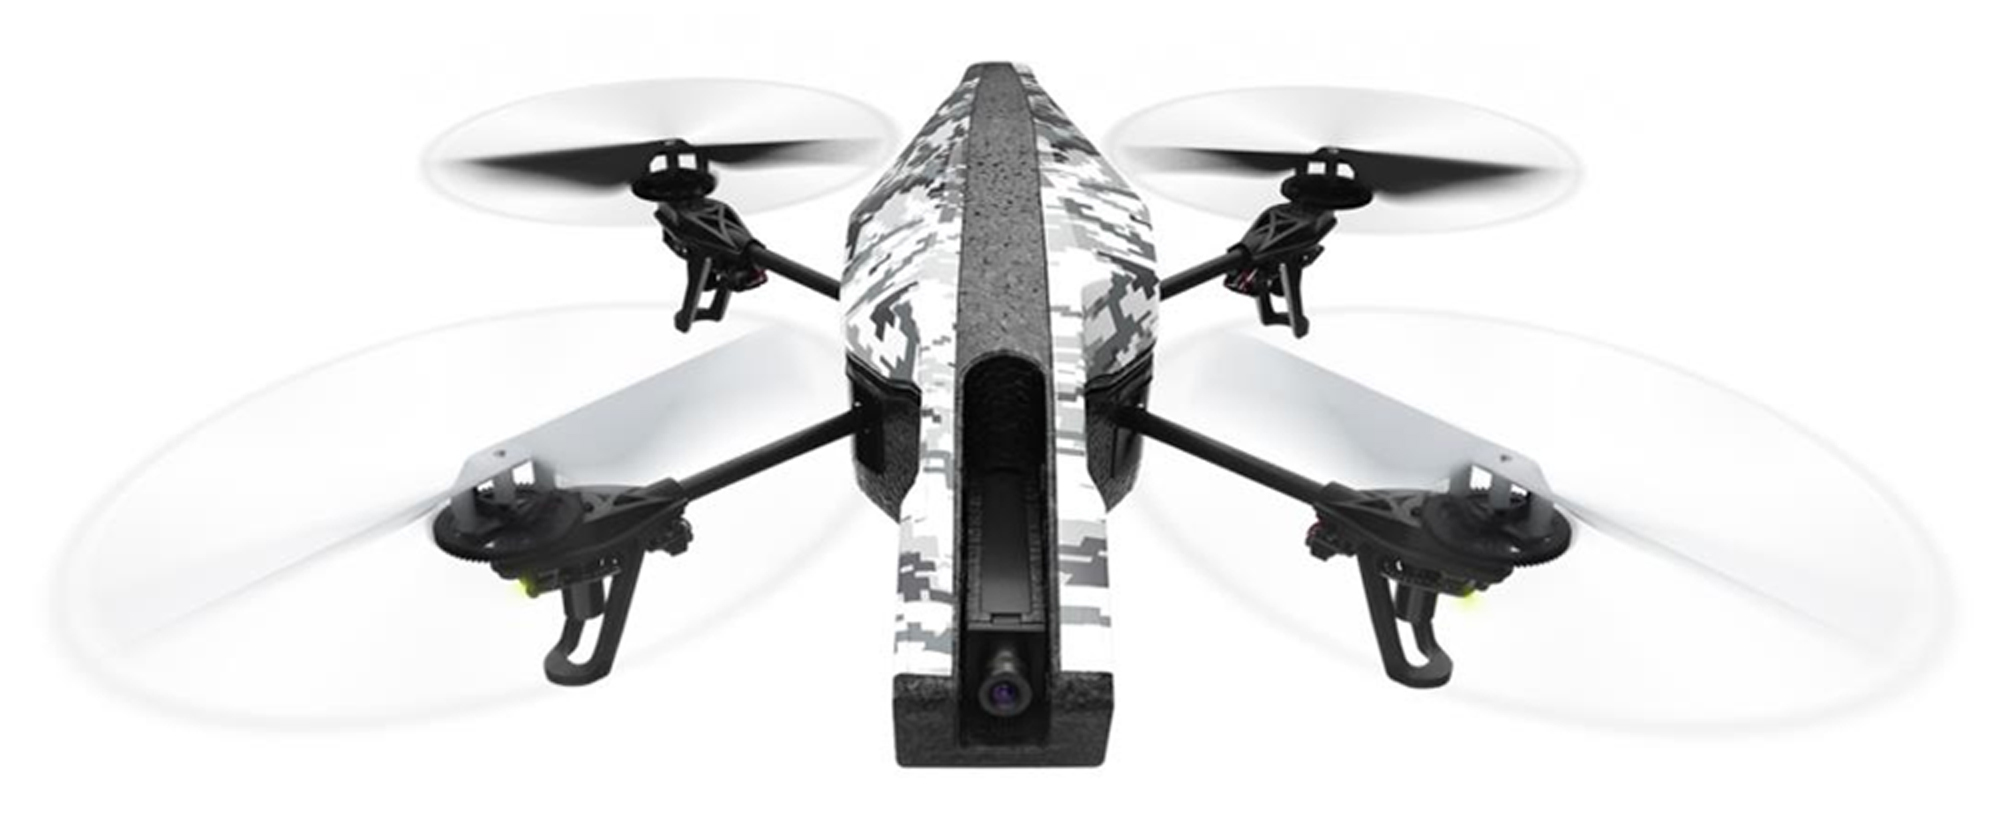
\includegraphics[width=0.7\textwidth]{images/ARDrone.jpg}
	\caption{Um \emph{AR.Drone}}
	\label{figARDrone}
\end{figure}

\section{Metodologia}

O controlador será baseado em algum controlador pré-existente. Estamos atualmente considerando 2 controladores: \emph{python-ardrone} \cite{pythonArdrone} e \emph{ardrone-autopylot} \cite{ardroneAutopylot}. A meta é adaptar um destes controladores para possibilitar um controle mais baixo-nível. A implementação será validada por via da constatação da execução exitosa de comandos de movimento.

Havendo sucesso no anterior, deseja-se construir um segundo controlador, baseado em um controle mais primitivo do hardware, que seja aprendido por uma rede neural. A priori, considera-se o uso de uma rede neural recorrente, junto a extratores de fatores latentes (e.g.: \emph{Convolutional Neural Networks}, \emph{Stacked Denoising Autoencoders}) para auxiliar na generalização do aprendizado. A rede receberá como entrada o estado do robô e uma representação do comando do usuário, e gerará como saída uma sequencia de ações a serem executadas pelo hardware do robô. Adotaremos um protocolo de aprendizado dividido em duas fases, em que (1) primeiro usamos aprendizado supervisionado para mapear as entradas (comando $\times$ estado $\rightarrow$ ação), durante o controle do robô por um humano, e (2) aprendizado por reforço, quando a rede neural pré treinada é posta a controlar o robô. 

Em paralelo a isto, novamente na condição de não houverem imprevistos na implementação do controlador em \emph{python}, propõe-se uma demonstração deste controlador por via de um experimento simples de localização. Estamos considerando 2 métodos de mapeamento para possibilitar a localização do robô: uso de marcadores coloridos ou relacionar localidades a fotos em arranjos tridimensionais (parecido com o que o \emph{google street view faz}). O algoritmo de localização em si será probabilístico e ainda não foi definido.

\section{Cronograma}

\begin{tabular}{c | p{10cm}}
	\textbf{19/10 - 25/10} 
	& Familiarização com a API/Protocolos do drone\\
	& Pesquisa bibliográfica\\
	\hline	
	\textbf{26/10 - 01/11} 
	& Controlador em python\\
	& Testes e depuração\\
	\hline		
	\textbf{02/11 - 08/11} 
	& (assumindo êxito no anterior)\\
	& Controlador por rede neural (André)\\
	& Localização com câmera (Jean Luc)\\
	\hline		
	\textbf{09/11 - 10/11} 
	& Elaboração da apresentação do trabalho\\	
	\hline		
	\textbf{11/11 ou 13/11}
	& Apresentação do trabalho\\
\end{tabular}


\begin{thebibliography}{99}

\bibitem{pythonArdrone}
	Projeto \emph{pythonArdrone}\\
	\url{https://github.com/venthur/python-ardrone}

\bibitem{ardroneAutopylot}
	Projeto \emph{ardroneAutopylot}\\
	\url{http://home.wlu.edu/~levys/software/ardrone\_autopylot/}

\bibitem{ardrone}
	Página oficial do \emph{AR.Drone}\\
	\url{http://ardrone2.parrot.com}

\end{thebibliography}

\end{document}

